\documentclass[10pt]{article}
\usepackage[a4paper,margin=18mm]{geometry}
\usepackage{amsmath,amssymb,booktabs,array,enumitem}
\usepackage[T1]{fontenc}\usepackage{lmodern}
\usepackage{tikz}\usetikzlibrary{shapes.gates.logic.US,positioning,arrows.meta,patterns,calc}
\usepackage[hidelinks]{hyperref}
\setlength{\parindent}{0pt}\setlength{\parskip}{4pt}
\setlength{\emergencystretch}{2em}
\newcommand{\VDD}{V_{DD}}
\newcommand{\mos}[4]{\begin{scope}[shift={(#1,#2)}]
\draw (0,.24)--(0,-.24);\draw (0,.20)--(.25,.20)--(.25,.5);
\draw (0,-.20)--(.25,-.20)--(.25,-.5);\draw (-.16,.23)--(-.16,-.23);
\ifnum#4=1\draw (-.26,0) circle (.06);\draw (-.75,0)--(-.32,0);\else\draw (-.75,0)--(-.16,0);\fi
\node[anchor=east,font=\scriptsize] at (-.76,0) {$#3$};\end{scope}}
\newcommand{\ground}[2]{\draw (#1,#2)--(#1,{#2-.12});\draw ({#1-.17},{#2-.12})--({#1+.17},{#2-.12});\draw ({#1-.11},{#2-.20})--({#1+.11},{#2-.20});}
\newcommand{\rail}[3]{\draw (#1,#2)--(#1,{#2+.14});\node[above,font=\scriptsize] at (#1,{#2+.14}) {$#3$};}

\newcommand{\hmos}[4]{\begin{scope}[shift={(#1,#2)}]
\draw(-.24,0)--(.24,0);\draw(-.2,0)--(-.2,-.25)--(-.5,-.25);\draw(.2,0)--(.2,-.25)--(.5,-.25);
\draw(-.23,.16)--(.23,.16);
\ifnum#4=1\draw(0,.26)circle(.06);\draw(0,.32)--(0,.75);\else\draw(0,.16)--(0,.75);\fi
\node[below,font=\scriptsize]at(0,-.32){#3};\end{scope}}
% ORIGINAL_LAYOUT_A / ORIGINAL_LAYOUT_B: normalized literal source topology.
% SOLUTION_LAYOUT_A / SOLUTION_LAYOUT_B: labelled MOS schematics, 12 devices each.
% Requires TikZ. No external image, style library, or custom circuit symbol needed.
\newcommand{\VLSIDiff}[2]{\fill[black!17] (#1,-.14) rectangle (#2,.14);\draw (#1,-.14) rectangle (#2,.14);}
\newcommand{\VLSIContact}[2]{\fill (#1-.075,#2-.075) rectangle (#1+.075,#2+.075);}
\newcommand{\VLSIRail}[3]{\draw[line width=3pt,black!35] (#1,#3)--(#2,#3);\draw (#1,#3-.085)--(#2,#3-.085) (#1,#3+.085)--(#2,#3+.085);}
\newcommand{\OriginalLayoutA}{%
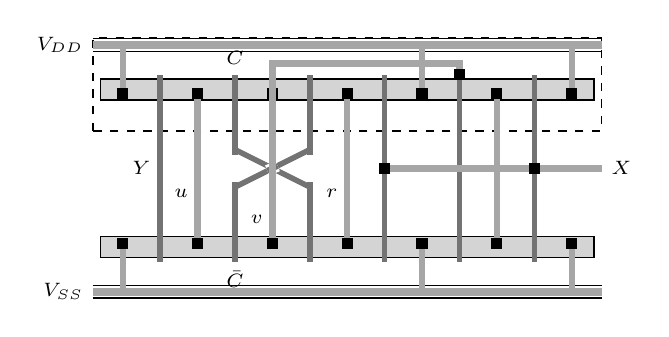
\begin{tikzpicture}[x=.95cm,y=.95cm,font=\scriptsize,line width=.5pt]
\draw[dashed] (-.4,.5) rectangle (6.4,1.75);
\begin{scope}[yshift=1cm]\VLSIDiff{-.3}{6.3}\end{scope}
\begin{scope}[yshift=-1cm]\VLSIDiff{-.3}{6.3}\end{scope}
\VLSIRail{-.4}{6.4}{1.65}\VLSIRail{-.4}{6.4}{-1.65}
\node[left] at (-.4,1.65) {$V_{DD}$};\node[left] at (-.4,-1.65) {$V_{SS}$};
% Six physical columns. Gate 1=Y; gate 2=C/Cbar; gate 3=Cbar/C;
% gate 4=X; gate 5=v; gate 6=X. Split clock gates are not shorted.
\foreach \x in {.5,3.5,4.5,5.5}{\draw[line width=2pt,black!55] (\x,-1.25)--(\x,1.25);}
\foreach \x in {1.5,2.5}{\draw[line width=2pt,black!55] (\x,.18)--(\x,1.25) (\x,-.18)--(\x,-1.25);}
\node[left] at (.5,0) {$Y$};\node[above] at (1.5,1.25) {$C$};\node[below] at (1.5,-1.25) {$\bar C$};
\draw[line width=2pt,black!55] (1.5,-.25)--(2.5,.25);\draw[line width=2pt,black!55] (1.5,.25)--(2.5,-.25);
% Opposite clock routes cross without a contact, shown with a bridge gap.
\draw[white,line width=4pt] (1.93,-.03)--(2.07,.03);\draw[line width=2pt,black!55] (1.93,-.03)--(2.07,.03);
% Supply contacts at physical channel intervals 0, 4, 6.
\foreach \x in {0,4,6}{\draw[line width=2.3pt,black!35] (\x,1)--(\x,1.65) (\x,-1)--(\x,-1.65);\VLSIContact{\x}{1}\VLSIContact{\x}{-1}}
% Inverter output u / transmission node v / feedback output r / X.
\foreach \x in {1,2,3,5}{\draw[line width=2.3pt,black!35] (\x,1)--(\x,-1);\VLSIContact{\x}{1}\VLSIContact{\x}{-1}}
\draw[line width=2.3pt,black!35] (2,.8)--(2,1.4)--(4.5,1.4)--(4.5,1.25);\VLSIContact{4.5}{1.25}
\draw[line width=2.3pt,black!35] (5,0)--(6.4,0) (3.5,0)--(5.5,0);\VLSIContact{3.5}{0}\VLSIContact{5.5}{0}
\node[right] at (6.4,0) {$X$};\node[below left] at (1,-.15) {$u$};\node[below left] at (2,-.5) {$v$};\node[below left] at (3,-.15) {$r$};
\end{tikzpicture}}
\newcommand{\OriginalLayoutB}{%
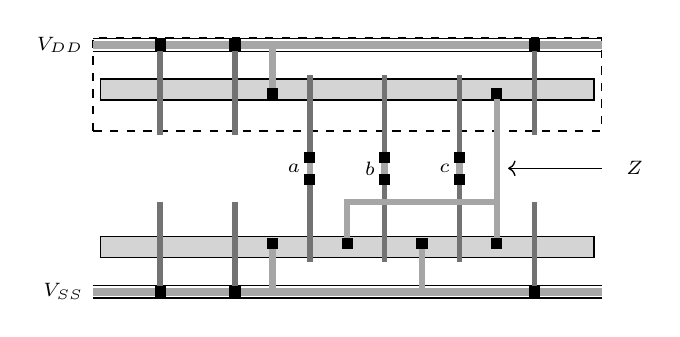
\begin{tikzpicture}[x=.95cm,y=.95cm,font=\scriptsize,line width=.5pt]
\draw[dashed] (-.4,.5) rectangle (6.4,1.75);
\begin{scope}[yshift=1cm]\VLSIDiff{-.3}{6.3}\end{scope}
\begin{scope}[yshift=-1cm]\VLSIDiff{-.3}{6.3}\end{scope}
\VLSIRail{-.4}{6.4}{1.65}\VLSIRail{-.4}{6.4}{-1.65}
\node[left] at (-.4,1.65) {$V_{DD}$};\node[left] at (-.4,-1.65) {$V_{SS}$};
\foreach \x in {.5,1.5,5.5}{\draw[line width=2pt,black!55] (\x,.45)--(\x,1.65) (\x,-.45)--(\x,-1.65);\VLSIContact{\x}{1.65}\VLSIContact{\x}{-1.65}}
\foreach \x/\g in {2.5/a,3.5/b,4.5/c}{\draw[line width=2pt,black!55] (\x,-1.25)--(\x,1.25);\draw[line width=2.3pt,black!35] (\x,-.15)--(\x,.15);\VLSIContact{\x}{-.15}\VLSIContact{\x}{.15}\node[left] at (\x,0) {$\g$};}
\draw[line width=2.3pt,black!35] (2,1)--(2,1.65) (2,-1)--(2,-1.65) (4,-1)--(4,-1.65);
\VLSIContact{2}{1}\VLSIContact{2}{-1}\VLSIContact{4}{-1}
\draw[line width=2.3pt,black!35] (5,1)--(5,-1) (3,-1)--(3,-.45)--(5,-.45);
\VLSIContact{5}{1}\VLSIContact{5}{-1}\VLSIContact{3}{-1}
\node[right] at (6.6,0) {$Z$};\draw[->] (6.4,0)--(5.15,0);
\end{tikzpicture}}

\newcommand{\SolutionLayoutA}{%
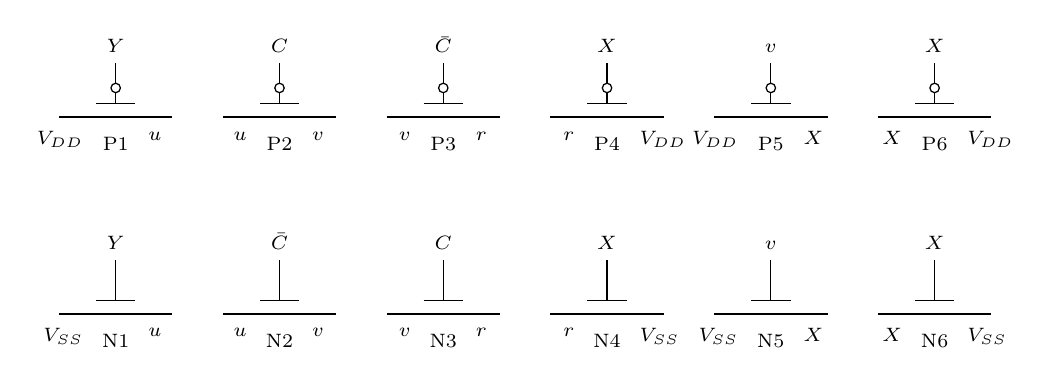
\begin{tikzpicture}[x=1cm,y=1cm,font=\scriptsize,line width=.45pt]
\draw (-0.72,2.5)--(-0.24,2.5) (0.24,2.5)--(0.72,2.5);
\draw[line width=1pt] (-0.24,2.5)--(0.24,2.5);
\draw (-0.25,2.67)--(0.25,2.67);
\draw (0.0,2.67)--(0.0,2.81);\draw (0.0,2.87) circle (.06);\draw (0.0,2.93)--(0.0,3.19);
\node[above] at (0.0,3.19) {$ Y $};
\node[below] at (0.0,2.37) {P1};
\node[anchor=north east] at (-0.29,2.44) {$ V_{DD} $};
\node[anchor=north west] at (0.29,2.44) {$ u $};
\draw (-0.72,0)--(-0.24,0) (0.24,0)--(0.72,0);
\draw[line width=1pt] (-0.24,0)--(0.24,0);
\draw (-0.25,0.17)--(0.25,0.17);
\draw (0.0,0.17)--(0.0,0.69);
\node[above] at (0.0,0.69) {$ Y $};
\node[below] at (0.0,-0.13) {N1};
\node[anchor=north east] at (-0.29,-0.06) {$ V_{SS} $};
\node[anchor=north west] at (0.29,-0.06) {$ u $};
\draw (1.36,2.5)--(1.84,2.5) (2.3200000000000003,2.5)--(2.8,2.5);
\draw[line width=1pt] (1.84,2.5)--(2.3200000000000003,2.5);
\draw (1.83,2.67)--(2.33,2.67);
\draw (2.08,2.67)--(2.08,2.81);\draw (2.08,2.87) circle (.06);\draw (2.08,2.93)--(2.08,3.19);
\node[above] at (2.08,3.19) {$ C $};
\node[below] at (2.08,2.37) {P2};
\node[anchor=north east] at (1.79,2.44) {$ u $};
\node[anchor=north west] at (2.37,2.44) {$ v $};
\draw (1.36,0)--(1.84,0) (2.3200000000000003,0)--(2.8,0);
\draw[line width=1pt] (1.84,0)--(2.3200000000000003,0);
\draw (1.83,0.17)--(2.33,0.17);
\draw (2.08,0.17)--(2.08,0.69);
\node[above] at (2.08,0.69) {$ \bar C $};
\node[below] at (2.08,-0.13) {N2};
\node[anchor=north east] at (1.79,-0.06) {$ u $};
\node[anchor=north west] at (2.37,-0.06) {$ v $};
\draw (3.4400000000000004,2.5)--(3.92,2.5) (4.4,2.5)--(4.88,2.5);
\draw[line width=1pt] (3.92,2.5)--(4.4,2.5);
\draw (3.91,2.67)--(4.41,2.67);
\draw (4.16,2.67)--(4.16,2.81);\draw (4.16,2.87) circle (.06);\draw (4.16,2.93)--(4.16,3.19);
\node[above] at (4.16,3.19) {$ \bar C $};
\node[below] at (4.16,2.37) {P3};
\node[anchor=north east] at (3.87,2.44) {$ v $};
\node[anchor=north west] at (4.45,2.44) {$ r $};
\draw (3.4400000000000004,0)--(3.92,0) (4.4,0)--(4.88,0);
\draw[line width=1pt] (3.92,0)--(4.4,0);
\draw (3.91,0.17)--(4.41,0.17);
\draw (4.16,0.17)--(4.16,0.69);
\node[above] at (4.16,0.69) {$ C $};
\node[below] at (4.16,-0.13) {N3};
\node[anchor=north east] at (3.87,-0.06) {$ v $};
\node[anchor=north west] at (4.45,-0.06) {$ r $};
\draw (5.5200000000000005,2.5)--(6.0,2.5) (6.48,2.5)--(6.96,2.5);
\draw[line width=1pt] (6.0,2.5)--(6.48,2.5);
\draw (5.99,2.67)--(6.49,2.67);
\draw (6.24,2.67)--(6.24,2.81);\draw (6.24,2.87) circle (.06);\draw (6.24,2.93)--(6.24,3.19);
\node[above] at (6.24,3.19) {$ X $};
\node[below] at (6.24,2.37) {P4};
\node[anchor=north east] at (5.95,2.44) {$ r $};
\node[anchor=north west] at (6.53,2.44) {$ V_{DD} $};
\draw (5.5200000000000005,0)--(6.0,0) (6.48,0)--(6.96,0);
\draw[line width=1pt] (6.0,0)--(6.48,0);
\draw (5.99,0.17)--(6.49,0.17);
\draw (6.24,0.17)--(6.24,0.69);
\node[above] at (6.24,0.69) {$ X $};
\node[below] at (6.24,-0.13) {N4};
\node[anchor=north east] at (5.95,-0.06) {$ r $};
\node[anchor=north west] at (6.53,-0.06) {$ V_{SS} $};
\draw (7.6000000000000005,2.5)--(8.08,2.5) (8.56,2.5)--(9.040000000000001,2.5);
\draw[line width=1pt] (8.08,2.5)--(8.56,2.5);
\draw (8.07,2.67)--(8.57,2.67);
\draw (8.32,2.67)--(8.32,2.81);\draw (8.32,2.87) circle (.06);\draw (8.32,2.93)--(8.32,3.19);
\node[above] at (8.32,3.19) {$ v $};
\node[below] at (8.32,2.37) {P5};
\node[anchor=north east] at (8.030000000000001,2.44) {$ V_{DD} $};
\node[anchor=north west] at (8.61,2.44) {$ X $};
\draw (7.6000000000000005,0)--(8.08,0) (8.56,0)--(9.040000000000001,0);
\draw[line width=1pt] (8.08,0)--(8.56,0);
\draw (8.07,0.17)--(8.57,0.17);
\draw (8.32,0.17)--(8.32,0.69);
\node[above] at (8.32,0.69) {$ v $};
\node[below] at (8.32,-0.13) {N5};
\node[anchor=north east] at (8.030000000000001,-0.06) {$ V_{SS} $};
\node[anchor=north west] at (8.61,-0.06) {$ X $};
\draw (9.68,2.5)--(10.16,2.5) (10.64,2.5)--(11.120000000000001,2.5);
\draw[line width=1pt] (10.16,2.5)--(10.64,2.5);
\draw (10.15,2.67)--(10.65,2.67);
\draw (10.4,2.67)--(10.4,2.81);\draw (10.4,2.87) circle (.06);\draw (10.4,2.93)--(10.4,3.19);
\node[above] at (10.4,3.19) {$ X $};
\node[below] at (10.4,2.37) {P6};
\node[anchor=north east] at (10.110000000000001,2.44) {$ X $};
\node[anchor=north west] at (10.69,2.44) {$ V_{DD} $};
\draw (9.68,0)--(10.16,0) (10.64,0)--(11.120000000000001,0);
\draw[line width=1pt] (10.16,0)--(10.64,0);
\draw (10.15,0.17)--(10.65,0.17);
\draw (10.4,0.17)--(10.4,0.69);
\node[above] at (10.4,0.69) {$ X $};
\node[below] at (10.4,-0.13) {N6};
\node[anchor=north east] at (10.110000000000001,-0.06) {$ X $};
\node[anchor=north west] at (10.69,-0.06) {$ V_{SS} $};
\end{tikzpicture}}
\newcommand{\SolutionLayoutB}{%
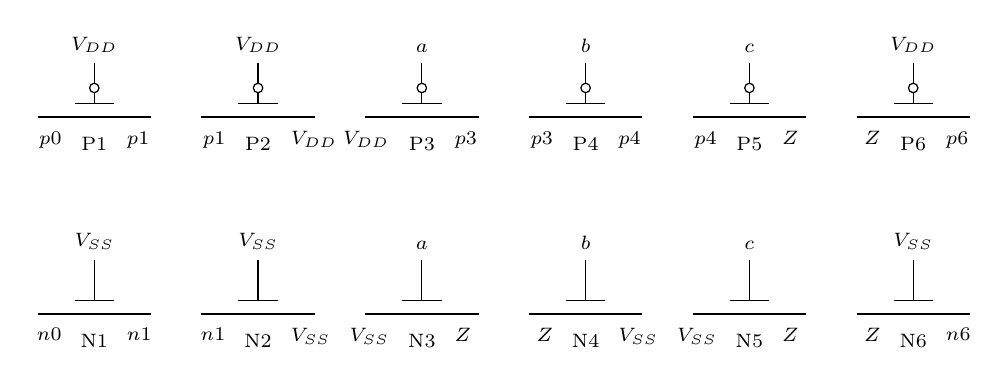
\begin{tikzpicture}[x=1cm,y=1cm,font=\scriptsize,line width=.45pt]
\draw (-0.72,2.5)--(-0.24,2.5) (0.24,2.5)--(0.72,2.5);
\draw[line width=1pt] (-0.24,2.5)--(0.24,2.5);
\draw (-0.25,2.67)--(0.25,2.67);
\draw (0.0,2.67)--(0.0,2.81);\draw (0.0,2.87) circle (.06);\draw (0.0,2.93)--(0.0,3.19);
\node[above] at (0.0,3.19) {$ V_{DD} $};
\node[below] at (0.0,2.37) {P1};
\node[anchor=north east] at (-0.29,2.44) {$ p0 $};
\node[anchor=north west] at (0.29,2.44) {$ p1 $};
\draw (-0.72,0)--(-0.24,0) (0.24,0)--(0.72,0);
\draw[line width=1pt] (-0.24,0)--(0.24,0);
\draw (-0.25,0.17)--(0.25,0.17);
\draw (0.0,0.17)--(0.0,0.69);
\node[above] at (0.0,0.69) {$ V_{SS} $};
\node[below] at (0.0,-0.13) {N1};
\node[anchor=north east] at (-0.29,-0.06) {$ n0 $};
\node[anchor=north west] at (0.29,-0.06) {$ n1 $};
\draw (1.36,2.5)--(1.84,2.5) (2.3200000000000003,2.5)--(2.8,2.5);
\draw[line width=1pt] (1.84,2.5)--(2.3200000000000003,2.5);
\draw (1.83,2.67)--(2.33,2.67);
\draw (2.08,2.67)--(2.08,2.81);\draw (2.08,2.87) circle (.06);\draw (2.08,2.93)--(2.08,3.19);
\node[above] at (2.08,3.19) {$ V_{DD} $};
\node[below] at (2.08,2.37) {P2};
\node[anchor=north east] at (1.79,2.44) {$ p1 $};
\node[anchor=north west] at (2.37,2.44) {$ V_{DD} $};
\draw (1.36,0)--(1.84,0) (2.3200000000000003,0)--(2.8,0);
\draw[line width=1pt] (1.84,0)--(2.3200000000000003,0);
\draw (1.83,0.17)--(2.33,0.17);
\draw (2.08,0.17)--(2.08,0.69);
\node[above] at (2.08,0.69) {$ V_{SS} $};
\node[below] at (2.08,-0.13) {N2};
\node[anchor=north east] at (1.79,-0.06) {$ n1 $};
\node[anchor=north west] at (2.37,-0.06) {$ V_{SS} $};
\draw (3.4400000000000004,2.5)--(3.92,2.5) (4.4,2.5)--(4.88,2.5);
\draw[line width=1pt] (3.92,2.5)--(4.4,2.5);
\draw (3.91,2.67)--(4.41,2.67);
\draw (4.16,2.67)--(4.16,2.81);\draw (4.16,2.87) circle (.06);\draw (4.16,2.93)--(4.16,3.19);
\node[above] at (4.16,3.19) {$ a $};
\node[below] at (4.16,2.37) {P3};
\node[anchor=north east] at (3.87,2.44) {$ V_{DD} $};
\node[anchor=north west] at (4.45,2.44) {$ p3 $};
\draw (3.4400000000000004,0)--(3.92,0) (4.4,0)--(4.88,0);
\draw[line width=1pt] (3.92,0)--(4.4,0);
\draw (3.91,0.17)--(4.41,0.17);
\draw (4.16,0.17)--(4.16,0.69);
\node[above] at (4.16,0.69) {$ a $};
\node[below] at (4.16,-0.13) {N3};
\node[anchor=north east] at (3.87,-0.06) {$ V_{SS} $};
\node[anchor=north west] at (4.45,-0.06) {$ Z $};
\draw (5.5200000000000005,2.5)--(6.0,2.5) (6.48,2.5)--(6.96,2.5);
\draw[line width=1pt] (6.0,2.5)--(6.48,2.5);
\draw (5.99,2.67)--(6.49,2.67);
\draw (6.24,2.67)--(6.24,2.81);\draw (6.24,2.87) circle (.06);\draw (6.24,2.93)--(6.24,3.19);
\node[above] at (6.24,3.19) {$ b $};
\node[below] at (6.24,2.37) {P4};
\node[anchor=north east] at (5.95,2.44) {$ p3 $};
\node[anchor=north west] at (6.53,2.44) {$ p4 $};
\draw (5.5200000000000005,0)--(6.0,0) (6.48,0)--(6.96,0);
\draw[line width=1pt] (6.0,0)--(6.48,0);
\draw (5.99,0.17)--(6.49,0.17);
\draw (6.24,0.17)--(6.24,0.69);
\node[above] at (6.24,0.69) {$ b $};
\node[below] at (6.24,-0.13) {N4};
\node[anchor=north east] at (5.95,-0.06) {$ Z $};
\node[anchor=north west] at (6.53,-0.06) {$ V_{SS} $};
\draw (7.6000000000000005,2.5)--(8.08,2.5) (8.56,2.5)--(9.040000000000001,2.5);
\draw[line width=1pt] (8.08,2.5)--(8.56,2.5);
\draw (8.07,2.67)--(8.57,2.67);
\draw (8.32,2.67)--(8.32,2.81);\draw (8.32,2.87) circle (.06);\draw (8.32,2.93)--(8.32,3.19);
\node[above] at (8.32,3.19) {$ c $};
\node[below] at (8.32,2.37) {P5};
\node[anchor=north east] at (8.030000000000001,2.44) {$ p4 $};
\node[anchor=north west] at (8.61,2.44) {$ Z $};
\draw (7.6000000000000005,0)--(8.08,0) (8.56,0)--(9.040000000000001,0);
\draw[line width=1pt] (8.08,0)--(8.56,0);
\draw (8.07,0.17)--(8.57,0.17);
\draw (8.32,0.17)--(8.32,0.69);
\node[above] at (8.32,0.69) {$ c $};
\node[below] at (8.32,-0.13) {N5};
\node[anchor=north east] at (8.030000000000001,-0.06) {$ V_{SS} $};
\node[anchor=north west] at (8.61,-0.06) {$ Z $};
\draw (9.68,2.5)--(10.16,2.5) (10.64,2.5)--(11.120000000000001,2.5);
\draw[line width=1pt] (10.16,2.5)--(10.64,2.5);
\draw (10.15,2.67)--(10.65,2.67);
\draw (10.4,2.67)--(10.4,2.81);\draw (10.4,2.87) circle (.06);\draw (10.4,2.93)--(10.4,3.19);
\node[above] at (10.4,3.19) {$ V_{DD} $};
\node[below] at (10.4,2.37) {P6};
\node[anchor=north east] at (10.110000000000001,2.44) {$ Z $};
\node[anchor=north west] at (10.69,2.44) {$ p6 $};
\draw (9.68,0)--(10.16,0) (10.64,0)--(11.120000000000001,0);
\draw[line width=1pt] (10.16,0)--(10.64,0);
\draw (10.15,0.17)--(10.65,0.17);
\draw (10.4,0.17)--(10.4,0.69);
\node[above] at (10.4,0.69) {$ V_{SS} $};
\node[below] at (10.4,-0.13) {N6};
\node[anchor=north east] at (10.110000000000001,-0.06) {$ Z $};
\node[anchor=north west] at (10.69,-0.06) {$ n6 $};
\end{tikzpicture}}

\begin{document}
\begin{center}{\large\bfseries Fall 2013 Final -- Independently Checked Solutions}\end{center}
\textbf{Scope and models.} All eight original questions are retained (150 printed points). The supplied handwritten work is ungraded and is compared only after derivation. The paper's single $R C$ approximation is used where specified. Q4 lacks external output loads, Q5 lacks separate gate minimum delays and a skew sign, and Q7 does not establish an upper trip voltage; those limits are stated where they affect an answer.

\textbf{1. Definitions and short answers.}
\begin{enumerate}[label=(\alph*),leftmargin=7mm,itemsep=4pt]
\item Use frequent, low-resistance well/substrate ties, and use guard rings to collect injected carriers. They reduce the well/substrate voltage rise and interrupt the parasitic PNPN regeneration responsible for latchup.
\item Physical design converts a circuit/netlist into manufacturable placement, geometries and interconnections. Instantiating a cell creates a named occurrence of a cell master and connects its pins. An instance is that individual occurrence; multiple instances can share one master.
\item Use the standard cell height, and align the VDD/VSS rail positions so adjacent cells can abut and share continuous rails. The layout must also satisfy the process design rules.
\item A soft error is a transient corruption of a stored or observed logic value, commonly caused by deposited charge, without permanent device damage.
\item \emph{Logical masking}: an upset does not reach a receiver if off-path inputs make the output independent of it; shorter/shallower critical paths and more observable paths can reduce this protection. \emph{Electrical masking}: a narrow pulse may attenuate through gates; smaller node charge and faster gates can increase pulse survival. \emph{Latch-window masking}: a surviving pulse matters only if it overlaps the sampling aperture; more clock edges per second increase exposure. These mechanisms explain the stated trend under comparable conditions; frequency alone does not prove that every circuit's soft-error rate increases monotonically.
\item Reduce shared supply/return inductance using more short VDD/VSS connections; reduce simultaneous-switching $|di/dt|$ using suitable output slew control or staggered switching. Since $\Delta V\simeq L\,di/dt$, both directly reduce bounce.
\item Charge sharing can lower a stored dynamic high, and direct same-phase dynamic cascades can irreversibly discharge a downstream node on a precharged upstream high. Leakage and input-noise sensitivity are further limitations.
\item Ordinary N-domino cascades implement noninverting functions; inversion needs another architecture or phase. Evaluation inputs must be monotonic (typically low-to-high), because a dynamic node cannot recharge after an erroneous discharge within that evaluation phase.
\item A core-limited die is sized mainly by its core logic and routing. A pad-limited die is sized mainly by pad count and required pad pitch/perimeter, potentially leaving unused core area.
\item With an always-on PMOS, a logic-low output involves NMOS/PMOS contention. The low voltage and noise margin depend on the pull-up/pull-down strength ratio, so correct levels require transistor ratios.
\end{enumerate}
\textbf{Student comparison.} The physical-design definition should describe layout implementation, not the wafer-manufacturing flow. ``Needs a buffer'' is a domino structural feature; it does not replace explaining the monotonic-evaluation limitation.

\newpage\textbf{2. Dynamic and fully differential implementations.}
Let $h=AB(C+D)$, so $f=\bar h=\bar A+\bar B+\bar C\bar D$. The same named terminal in the following MOS schematics denotes one electrical net; each gate and both channel terminals are explicitly given.
\begin{center}\begin{tikzpicture}[x=.8cm,y=.82cm,font=\scriptsize]
\mos{0}{0.0}{\phi}{1}\node[right]at(0.45,0.45){$\mathrm{Ppre}$};\node[above]at(0.25,0.5){$V_{DD}$};\node[below]at(0.25,-0.5){$f$};
\mos{5}{0.0}{A}{0}\node[right]at(5.45,0.45){$\mathrm{NA}$};\node[above]at(5.25,0.5){$f$};\node[below]at(5.25,-0.5){$u$};
\mos{10}{0.0}{B}{0}\node[right]at(10.45,0.45){$\mathrm{NB}$};\node[above]at(10.25,0.5){$u$};\node[below]at(10.25,-0.5){$v$};
\mos{0}{-2.25}{C}{0}\node[right]at(0.45,-1.8){$\mathrm{NC}$};\node[above]at(0.25,-1.75){$v$};\node[below]at(0.25,-2.75){$w$};
\mos{5}{-2.25}{D}{0}\node[right]at(5.45,-1.8){$\mathrm{ND}$};\node[above]at(5.25,-1.75){$v$};\node[below]at(5.25,-2.75){$w$};
\mos{10}{-2.25}{\phi}{0}\node[right]at(10.45,-1.8){$\mathrm{Nclk}$};\node[above]at(10.25,-1.75){$w$};\node[below]at(10.25,-2.75){$0$};
\end{tikzpicture}\end{center}
\textbf{Dynamic (6 transistors).} At $\phi=0$, Ppre charges $f$ high and Nclk disconnects ground. At $\phi=1$, the NMOS network discharges $f$ exactly when $h=1$. The raw dynamic output already is the requested complemented function; adding an inverter would change it to $h$.
\begin{center}\begin{tikzpicture}[x=.8cm,y=.82cm,font=\scriptsize]
\mos{0}{0.0}{\bar f}{1}\node[right]at(0.45,0.45){$\mathrm{Pf}$};\node[above]at(0.25,0.5){$V_{DD}$};\node[below]at(0.25,-0.5){$f$};
\mos{5}{0.0}{f}{1}\node[right]at(5.45,0.45){$\mathrm{Pg}$};\node[above]at(5.25,0.5){$V_{DD}$};\node[below]at(5.25,-0.5){$\bar f$};
\mos{10}{0.0}{A}{0}\node[right]at(10.45,0.45){$\mathrm{NA}$};\node[above]at(10.25,0.5){$f$};\node[below]at(10.25,-0.5){$u$};
\mos{0}{-2.25}{B}{0}\node[right]at(0.45,-1.8){$\mathrm{NB}$};\node[above]at(0.25,-1.75){$u$};\node[below]at(0.25,-2.75){$v$};
\mos{5}{-2.25}{C}{0}\node[right]at(5.45,-1.8){$\mathrm{NC}$};\node[above]at(5.25,-1.75){$v$};\node[below]at(5.25,-2.75){$0$};
\mos{10}{-2.25}{D}{0}\node[right]at(10.45,-1.8){$\mathrm{ND}$};\node[above]at(10.25,-1.75){$v$};\node[below]at(10.25,-2.75){$0$};
\mos{0}{-4.5}{\bar A}{0}\node[right]at(0.45,-4.05){$\mathrm{Na}$};\node[above]at(0.25,-4.0){$\bar f$};\node[below]at(0.25,-5.0){$0$};
\mos{5}{-4.5}{\bar B}{0}\node[right]at(5.45,-4.05){$\mathrm{Nb}$};\node[above]at(5.25,-4.0){$\bar f$};\node[below]at(5.25,-5.0){$0$};
\mos{10}{-4.5}{\bar C}{0}\node[right]at(10.45,-4.05){$\mathrm{Nc}$};\node[above]at(10.25,-4.0){$\bar f$};\node[below]at(10.25,-5.0){$w$};
\mos{0}{-6.75}{\bar D}{0}\node[right]at(0.45,-6.3){$\mathrm{Nd}$};\node[above]at(0.25,-6.25){$w$};\node[below]at(0.25,-7.25){$0$};
\end{tikzpicture}\end{center}
\textbf{Fully differential (10-transistor core).} One NMOS network realizes $h$ under $f$, and the other realizes $\bar h$ under $\bar f$. The two PMOS loads are cross-coupled to the opposite output. If complementary primary inputs are unavailable, add four ordinary CMOS inverters (8 transistors), giving 18 in total. Their complementary inputs are assumptions of the core diagram, not floating terminals. Exactly one pull-down network conducts for every binary ABCD, so the stable outputs are complementary and full swing.
\textbf{Student comparison.} The printed function has a single bar over the whole $AB(C+D)$. Fully differential logic uses cross-coupled PMOS loads directly; reference-biased clamp transistors of differential split-level logic do not belong here.

\newpage\textbf{3. Balanced domino widths.}
\begin{center}\begin{tikzpicture}[scale=.83,font=\scriptsize]
\mos{2}{5}{CLK}{1}\rail{2.25}{5.5}{V_{DD}}\node[right]at(2.6,5){P1};\draw(.25,4.5)--(4.25,4.5);\node[above]at(3,4.5){$X$};
\mos{0}{3}{}{0}\node[right]at(.45,3){N1};\draw(.25,3.5)--(.25,4.5);\draw(.25,2.5)--(.25,1.5);
\mos{2}{4}{}{0}\mos{2}{2}{}{0}\node[right]at(2.55,4){N2};\node[right]at(2.55,2){N3};\draw(2.25,3.5)--(2.25,2.5);
\mos{4}{4}{}{0}\mos{4}{3}{}{0}\node[right]at(4.6,4){N4};\node[right]at(4.6,3){N5};\draw(2.25,2.5)--(4.25,2.5);\fill(2.25,2.5)circle(1pt);
\draw(.25,1.5)--(2.25,1.5);\mos{2}{1}{CLK}{0}\node[right]at(2.6,1){N6};\ground{2.25}{.5}
\mos{7}{4.1}{}{1}\mos{7}{3.1}{}{0}\rail{7.25}{4.6}{V_{DD}}\ground{7.25}{2.6}\node[right]at(7.6,4.1){P2};\node[right]at(7.6,3.1){N7};\draw(4.25,4.5)--(5.8,4.5)--(5.8,3.1)--(6.25,3.1);\draw(5.8,4.1)--(6.25,4.1);\draw(7.25,3.6)--(8.4,3.6)node[right]{output};\end{tikzpicture}\end{center}
The shared N3 connection is essential: the discharge alternatives are N1--N6, N2--N3--N6, and N4--N5--N3--N6. It is not a pair of independent two-device branches. With common length, write $R_N=k/W_N$ and $R_{P1}=3k/W_P$. Equal delay means matching the \emph{worst-case single conducting path}; additional simultaneous paths reduce fall time and cannot make every input pattern have exactly the same delay.
\[
\frac1{W_1}+\frac1{W_6}=\frac1{W_2}+\frac1{W_3}+\frac1{W_6}
=\frac1{W_4}+\frac1{W_5}+\frac1{W_3}+\frac1{W_6}=\frac3{W_P}.
\]
A convenient valid family is $W_P=W_6=s$, $W_1=s/2$, $W_2=W_3=s$, and $W_4=W_5=2s$. All three path resistances equal $3k/s$.
\begin{center}\begin{tabular}{c*{7}{c}}\toprule
Part & P1 & N1 & N2 & N3 & N4 & N5 & N6\\\midrule
(a), width ($\mu$m)&4&2&4&4&8&8&4\\
(b), width ($\mu$m)&2&1&2&2&4&4&2\\\bottomrule
\end{tabular}\\All channel lengths are $0.18\,\mu$m.\end{center}
\textbf{(b) Clock loading.} CLK drives P1 and N6 only. A $2\,\mu$m device contributes $C$, so
\[
C_{CLK}=C\frac{W_P+W_6}{2\,\mu\mathrm m},\qquad P_{CLK}=fC_{CLK}V_{DD}^{2}.
\]
The printed $2fCV_{DD}^{2}$ therefore requires $W_P+W_6=4\,\mu$m, met by the second row. There is one supply charging event per full clock cycle; counting both edges as separate $CV^2$ supply charges incorrectly doubles the power.
\textbf{Nonuniqueness and student comparison.} No area or common-width optimum is requested, so these equations have many solutions. The student's part (a) widths $W_1=16/9$, $W_2=8/3$, and $W_3=W_4=W_5=W_6=16/3$ ($\mu$m), with $W_P=4$, are also valid: each path is $3k/4$. This is accepted after checking all three paths. The student's part (b) annotations are not a reason to replace the explicit clock-capacitance equation.

\newpage\textbf{4. NP-domino timing and charge sharing.}
\begin{center}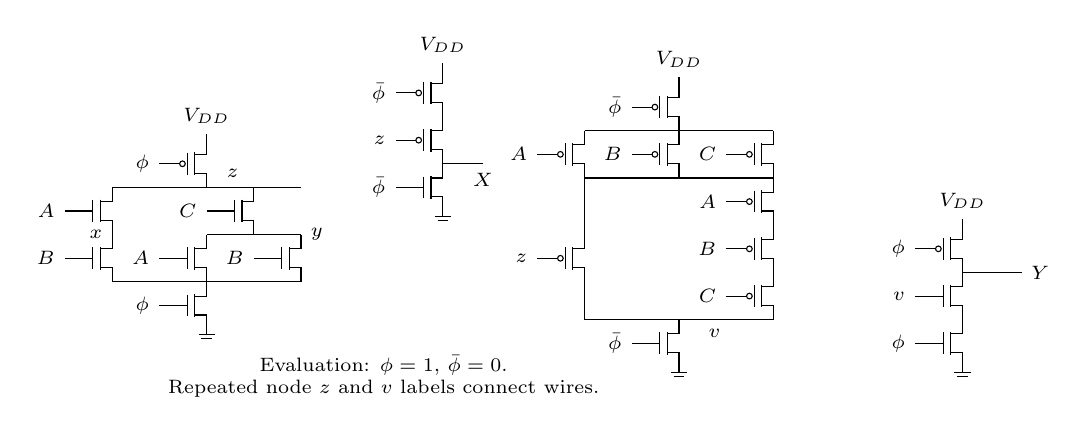
\begin{tikzpicture}[scale=.60,font=\scriptsize]
\mos{2}{5.8}{\phi}{1}\rail{2.25}{6.3}{V_{DD}}\draw(.25,5.3)--(4.25,5.3);\node[above]at(2.8,5.3){$z$};
\mos{0}{4.8}{A}{0}\mos{0}{3.8}{B}{0}\node[left]at(.25,4.3){$x$};\mos{3}{4.8}{C}{0}\draw(3.25,4.3)--(4.25,4.3);\mos{2}{3.8}{A}{0}\mos{4}{3.8}{B}{0}\draw(2.25,4.3)--(3.25,4.3);\node[right]at(4.25,4.3){$y$};\draw(.25,3.3)--(4.25,3.3);\mos{2}{2.8}{\phi}{0}\ground{2.25}{2.3}
\mos{7}{7.3}{\bar\phi}{1}\rail{7.25}{7.8}{V_{DD}}\mos{7}{6.3}{z}{1}\mos{7}{5.3}{\bar\phi}{0}\ground{7.25}{4.8}\draw(7.25,5.8)--(8.1,5.8)node[below]{$X$};
\mos{12}{7}{\bar\phi}{1}\rail{12.25}{7.5}{V_{DD}}\draw(10.25,6.5)--(14.25,6.5);\mos{10}{6}{A}{1}\mos{12}{6}{B}{1}\mos{14}{6}{C}{1}\draw(10.25,5.5)--(14.25,5.5);
\mos{10}{3.8}{z}{1}\draw(10.25,4.3)--(10.25,5.5);\draw(10.25,3.3)--(10.25,2.5)--(14.25,2.5);
\mos{14}{5}{A}{1}\mos{14}{4}{B}{1}\mos{14}{3}{C}{1}\mos{12}{2}{\bar\phi}{0}\ground{12.25}{1.5}\node[below]at(13,2.5){$v$};
\mos{18}{4}{\phi}{1}\rail{18.25}{4.5}{V_{DD}}\mos{18}{3}{v}{0}\mos{18}{2}{\phi}{0}\ground{18.25}{1.5}\draw(18.25,3.5)--(19.5,3.5)node[right]{$Y$};
\node[align=center]at(6,1.3){Evaluation: $\phi=1$, $\bar\phi=0$.\\Repeated node $z$ and $v$ labels connect wires.};\end{tikzpicture}\end{center}
For evaluation, $\phi=1$ and $\bar\phi=0$. Let $M=AB+C(A+B)$. The first dynamic node is $z=\bar M$; the P dynamic output $X$ is $M$. The middle pull-up condition is
\[
v=(\bar A+\bar B+\bar C)\bigl(\bar z+\bar A\bar B\bar C\bigr)
=\overline{A\oplus B\oplus C},\qquad Y=\bar v=A\oplus B\oplus C.
\]
The middle $z$ transistor is \emph{after} the three parallel input PMOS. Its branch does not bypass those three transistors. The final PMOS is clock-controlled, so $v$ drives only the final NMOS gate.

\textbf{(a) State-correlated RC calculation.} Neglecting drain capacitance gives $C_z=4C$ (two PMOS gates), $C_v=C$ (one NMOS gate). Denote unspecified external capacitances at $X,Y$ by $C_X,C_Y$. Each end gate has precharge resistance $R$ and evaluation resistance $2R$, hence average delay $3RC_X/2$ or $3RC_Y/2$.
\begin{center}\begin{tabular}{llll}\toprule
Node and input state & Evaluation resistance & Precharge resistance & Average delay\\\midrule
$z$, exactly two ones & $3R$ & $R$ & $8RC$\\
$z$, three ones & $R+(2R\parallel\tfrac32R)=\tfrac{13}{7}R$ & $R$ & $\tfrac{40}{7}RC$\\
$v$, zero ones & $R+R/3+3R=\tfrac{13}{3}R$ & $R$ & $\tfrac83RC$\\
$v$, exactly two ones & $3R$ & $R$ & $2RC$\\\bottomrule\end{tabular}\end{center}
The $z\to v$ path is sensitized only with exactly two ones. Thus the feasible complete path estimates are
\[
\begin{array}{ll}
\text{fastest }z\to X:&\tfrac{40}{7}RC+\tfrac32RC_X,\\
\text{slowest }z\to X:&8RC+\tfrac32RC_X,\\
\text{direct inputs}\to v\to Y\;(000):&\tfrac83RC+\tfrac32RC_Y,\\
\text{inputs}\to z\to v\to Y\;(\text{two ones}):&10RC+\tfrac32RC_Y.
\end{array}
\]
Taking the minimum and maximum of these feasible paths gives $t_{cd}$ and $t_{pd}$ under the printed average-delay rule. For its literal unloaded limit $C_X=C_Y=0$,
\[\boxed{t_{cd}=\tfrac83RC,\quad t_{pd}=10RC.}\]
The zero end-gate delay here follows from the instructed omission of drain capacitance and absent external loads; it is a limit of that model, not a claim that real output nodes switch instantaneously. A conventional single-conducting-path count, which ignores parallel speed-up and input-state correlation, instead provides the looser local bounds $t_{cd}\geq2RC$ and $t_{pd}\leq11RC$ for the unloaded circuit. Summing incompatible local extrema does not establish an actual sensitized 11RC path.

\textbf{(b) It is not robustly correct.} Start with $z$ precharged to 1.8 V and an internal $y$ node at 0 V. Set $C=1,A=B=0$: there is no path to ground, but NC connects $z$ to $y$. Charge conservation gives
\[V_z'=\frac{C_z}{C_z+C_y}V_{DD}=\frac{1.0}{1.0+0.8}(1.8)=1.0\ \mathrm V.\]
The following PMOS can turn on when $V_z<V_{DD}-|V_{tp}|=1.3$ V. The droop to 1.0 V therefore falsely raises $X$, and can also raise $v$ and discharge $Y$. This one legal counterexample is sufficient. The $x$-only share gives $1.8/(1+0.4)=1.286$ V, also below 1.3 V. Summing $C_x+C_y$ for a nonconducting state is unjustified: connecting both internal nodes requires A=C=1, which already makes the majority network conduct.
\textbf{Student comparison.} ``Same as 2012'' omits the solution and misses a material change: the 2013 $z$ capacitance is 1.0 pF, not the 2012 1.6 pF. The 2012 figure is used only to clarify identical connections.

\newpage\textbf{5. Setup, hold, skew and three-register retiming.}
From Figure 3, $u=\overline{A+B}$, $v=B\oplus C$, $w=A\oplus C$, $s=\overline{v\oplus\bar w}$, and the register inputs are $u$, $\overline{u\oplus s}$, $w$. Here A/B/C are R1/R2/R3 Q values. Use each printed gate delay as both minimum and maximum for the numerical exercise; actual separate gate contamination delays are not supplied.
With $\delta=t_{capture}-t_{launch}$, the exact sign convention is
\[T\geq t_{pcq}+d_{max}+t_{setup}-\delta,\qquad
t_{ccq}+d_{min}\geq t_{hold}+\delta.\]
\textbf{(a)} The NOR path to R4 has $t_{ccq}+d_{min}=0.1+0.2=0.3$ ns $<0.4$ ns, a hold violation. Put a noninverting delay of at least 0.1 ns in \emph{only} the branch from NOR output to R4. Two printed inverters give 0.4 ns and preserve polarity. Its new data delay is 0.6 ns, below the 1.5 ns critical path, so this repair does not lower the maximum frequency.

\textbf{(b)} The longest path is XOR--INV--XNOR--XNOR:
\[d_{max}=0.5+0.2+0.4+0.4=1.5\ \mathrm{ns},\quad
T_{min}=0.3+1.5+0.2=2.0\ \mathrm{ns},\quad\boxed{f_{max}=500\ \mathrm{MHz}.}\]
This is a working frequency after the hold repair; a setup-only number does not make the original unmodified circuit valid.

\textbf{(c)} A skew magnitude has no sign. With an adverse 0.5 ns early capture clock ($\delta=-0.5$), $T_{min}=2.5$ ns and $f_{max}=400$ MHz. With a 0.5 ns late capture clock ($\delta=+0.5$), the setup-only bound is 1.5 ns / 666.7 MHz, but the hold requirement rises to $d_{min}\geq0.8$ ns. Local noninverting padding of the R4 branch (four INV), R6 branch (two INV), and the NOR-to-last-XNOR branch (two INV) can satisfy this without exceeding the existing 1.5 ns maximum. Thus the 666.7 MHz case needs those hold repairs. For unspecified skew with $|\delta|\leq0.5$ ns, design hold for late capture and setup for early capture, yielding a robust 400 MHz bound. The student's 400 MHz value is valid for adverse/bounded skew, not a proof of the sign.

\textbf{(d) Exactly three additional registers.} Insert one after NOR, one after the middle XOR, and one after the lower inverter. The stored signals are $u$, $v$ and $\bar w$, so both inputs of the remaining XNOR cascade have the same age. The first-stage maximum is $0.5+0.2=0.7$ ns and the second is $0.4+0.4=0.8$ ns. At zero skew,
\[\boxed{d_{max,stage}=0.8\ \mathrm{ns},\quad T_{min}=0.3+0.8+0.2=1.3\ \mathrm{ns},\quad f_{max}=769.23\ \mathrm{MHz}.}\]
The new NOR FF needs its hold repair (two INV, total 0.6 ns). The stage-two bypass to R4 needs two INV (0.4 ns). R6 needs one inverter to restore $w$ from stored $\bar w$; two more inverters give a hold-safe total of 0.6 ns. All these paths remain below 0.8 ns. Each output gains one cycle of latency, with Boolean values aligned.
\begin{center}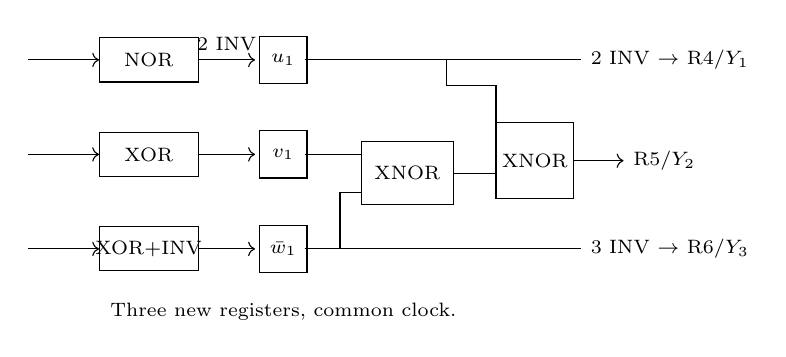
\begin{tikzpicture}[x=.9cm,y=.8cm,font=\scriptsize]
\foreach\y/\g/\q in {3/NOR/$u_1$,1.5/XOR/$v_1$,0/XOR+INV/$\bar w_1$}{\draw[->](0,\y)--(1,\y);\draw(1,\y-.35)rectangle(2.4,\y+.35);\node at(1.7,\y){\g};\draw[->](2.4,\y)--(3.2,\y);\node[draw,minimum width=.6cm,minimum height=.6cm]at(3.6,\y){\q};}\node[above]at(2.8,3){2 INV};
\draw(3.9,3)--(7.8,3)node[right]{2 INV $\to$ R4/$Y_1$};\draw(3.9,1.5)--(4.7,1.5);\draw(3.9,0)--(4.4,0)--(4.4,.9)--(4.7,.9);\draw(4.7,.7)rectangle(6.0,1.7);\node at(5.35,1.2){XNOR};\draw(6,1.2)--(6.6,1.2);\draw(6.6,.8)rectangle(7.7,2);\node at(7.15,1.4){XNOR};\draw(5.9,3)--(5.9,2.6)--(6.6,2.6)--(6.6,1.8);\draw[->](7.7,1.4)--(8.4,1.4)node[right]{R5/$Y_2$};\draw(3.9,0)--(7.8,0)node[right]{3 INV $\to$ R6/$Y_3$};\node[below]at(3.6,-.7){Three new registers, common clock.};\end{tikzpicture}\end{center}
With fixed gates and aligned output latency, the NOR branch must be registered and the lower branch must have one cut before or after its inverter (the latter requires restoration). Cutting each reconvergent branch before the first XNOR leaves 1.0 ns if the lower cut is before INV, or 0.8 ns if after it. Moving the common cut after the first XNOR instead requires a 1.1 ns first stage. Moving it after the last requires 1.5 ns. These possible aligned frontiers establish the 0.8 ns optimum under the stated three-FF budget. The student's first-level cut gives a valid 1.5 ns clock, but does not maximize improvement. A 1.0 ns clock would require more FFs or a functional logic redesign.

\newpage\textbf{6. Contact-extracted transistor schematics.}
\textbf{(a) Literal 12-MOS extraction.} The original has two TG pairs, three ordinary inverter pairs and a final self-connected pair. The last P6/N6 have gate X and channel X--VDD / X--VSS, respectively. At binary-low X, P6 opposes that low; at binary-high X, N6 opposes that high. Preserve these connections rather than silently replacing them with a conventional inverter or asserting an ordinary functioning latch.
\begin{center}\SolutionLayoutA\end{center}
\textbf{(b) Literal 12-MOS extraction.} The central a,b,c devices form three series PMOS and three parallel NMOS, giving $Z=\overline{a+b+c}$. The six remaining devices (columns 1,2,6) have PMOS gates tied to VDD / NMOS gates tied to VSS and remain OFF. Their floating active-strip stubs are retained explicitly; they do not add an input inverter.
\begin{center}\SolutionLayoutB\end{center}
The original vector layouts normalize geometry, retaining each physical crossing, contact and split gate. They are connectivity reconstructions, not mask-scale manufacturing layouts. Twelve physical MOS are counted in each even where OFF devices can be omitted from a functional Boolean reduction.
The connections, not a remembered gate shape or the student's sketches, determine the functions. Identical high-resolution 2012 source layouts were used to read contacts that are tiny in the 2013 photographs; they do not replace the 2013 question. The extracted device lists and all-input connectivity checks are saved beside this document.

\newpage\textbf{7. What the waveform establishes about hysteresis.}
\begin{center}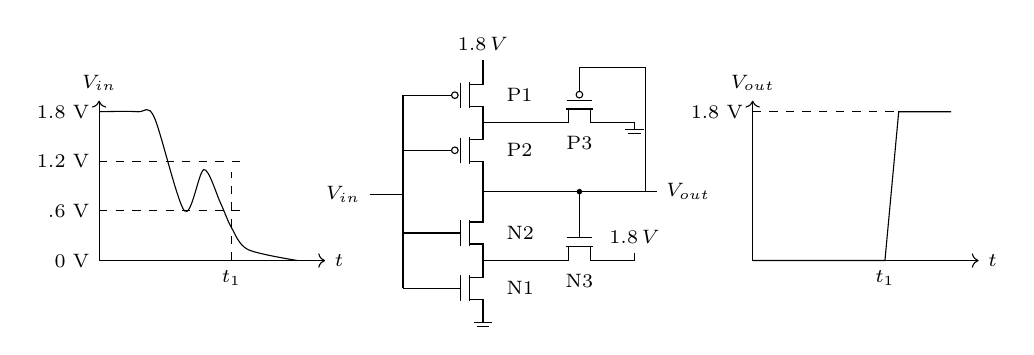
\begin{tikzpicture}[x=.7cm,y=.7cm,font=\scriptsize]
\draw[->](0,0)--(4.1,0)node[right]{$t$};\draw[->](0,0)--(0,2.9)node[above]{$V_{in}$};\foreach\y/\v in {0/0,.9/.6,1.8/1.2,2.7/1.8}{\node[left]at(0,\y){$\v$ V};}\draw[dashed](0,.9)--(2.6,.9);\draw[dashed](0,1.8)--(2.6,1.8);\draw plot[smooth]coordinates{(0,2.7)(.7,2.7)(1,2.6)(1.55,.9)(1.9,1.65)(2.2,1.05)(2.4,.6)(2.7,.2)(3.6,0)};\draw[dashed](2.4,0)--(2.4,1.6);\node[below]at(2.4,0){$t_1$};
\begin{scope}[xshift=4cm]\mos{1}{3}{}{1}\mos{1}{2}{}{1}\mos{1}{.5}{}{0}\mos{1}{-.5}{}{0}\rail{1.25}{3.5}{1.8\,V}\ground{1.25}{-1}\draw(1.25,1)--(1.25,1.5);\draw(1.25,1.25)--(4.4,1.25)node[right]{$V_{out}$};\draw(-.2,-.5)--(-.2,3)--(.25,3);\foreach\y in {2,.5,-.5}{\draw(-.2,\y)--(.25,\y);}\draw(-.8,1.2)node[left]{$V_{in}$}--(-.2,1.2);\node[right]at(1.5,3){P1};\node[right]at(1.5,2){P2};\node[right]at(1.5,.5){N2};\node[right]at(1.5,-.5){N1};
\hmos{3}{2.75}{P3}{1}\draw(1.25,2.5)--(2.5,2.5);\draw(3.5,2.5)--(4,2.5);\ground{4}{2.5}\draw(3,3.5)--(4.2,3.5)--(4.2,1.25);\hmos{3}{.25}{N3}{0}\draw(1.25,0)--(2.5,0);\draw(3.5,0)--(4,0);\rail{4}{0}{1.8\,V}\draw(3,1)--(3,1.25);\fill(3,1.25)circle(1pt);\end{scope}
\begin{scope}[xshift=8.3cm]\draw[->](0,0)--(4.1,0)node[right]{$t$};\draw[->](0,0)--(0,2.9)node[above]{$V_{out}$};\node[left]at(0,2.7){1.8 V};\draw[dashed](0,2.7)--(3.3,2.7);\draw(0,0)--(2.4,0)--(2.65,2.7)--(3.6,2.7);\node[below]at(2.4,0){$t_1$};\end{scope}\end{tikzpicture}\end{center}
The input falls, bounces to an intermediate peak and falls again. The output stays low through the first trough and rises only at $t_1$. There is no demonstrated high-to-low output transition on a rising input. In particular, the 1.2 V line labels the rebound amplitude; it does \emph{not} label the upper Schmitt trip voltage $V_T^+$. Substituting $V_T^+=1.2$ V is unsupported.

Let $L$ be the first trough. In a quasistatic interpretation, with enough time to settle, the unchanged low output requires $V_T^-\leq L\simeq0.6$ V if touching the threshold without crossing is allowed. If the dip is too brief, finite response time can mask it and even this bound is not compulsory. The final fall must cause the output to switch, but a scaled sketch and an output transition time do not determine an exact threshold in the presence of delay. The shown rebound occurs \emph{before} the output goes high, so it cannot measure the upper trip threshold. Ordinary hysteresis requires $V_T^+>V_T^-$.

\textbf{Long-channel threshold model.} Neglect body effect and channel-length modulation, assume rail outputs immediately before switching, and use the conventional onset condition for the stacked N2/P2. On the rising input, the N1--N3 internal node is $V_T^+-V_{tn}$, giving
\[\beta_{N1}(V_T^+-V_{tn})^2=\beta_{N3}(V_{DD}-V_T^+)^2,
\quad\boxed{\frac{\beta_{N1}}{\beta_{N3}}=\left(\frac{1.8-V_T^+}{V_T^+-0.6}\right)^2}.\]
On the falling input, the P1--P3 node is $V_T^-+|V_{tp}|$, giving
\[\beta_{P1}(V_{DD}-V_T^--|V_{tp}|)^2=\beta_{P3}(V_T^-)^2,
\quad\boxed{\frac{\beta_{P1}}{\beta_{P3}}=\left(\frac{V_T^-}{1.2-V_T^-}\right)^2}.\]
Under the quasistatic bound $0<V_T^-\leq0.6$ V, this gives $0<\beta_{P1}/\beta_{P3}\leq1$. If an ideal, delay-free interpretation explicitly identifies the lower crossing as exactly 0.6 V, the second ratio is 1; that extra interpretation still does not establish the first ratio.

\textbf{Fixed-resistance classroom approximation.} If one instead treats on-resistances as constants and sets the stacked device to turn on at its threshold, the divider equations give
\[
V_T^+=V_{tn}+\frac{V_{DD}}{1+\beta_{N1}/\beta_{N3}},\quad
V_T^-=V_{DD}-|V_{tp}|-\frac{V_{DD}}{1+\beta_{P1}/\beta_{P3}}.
\]
These are approximate divider formulas with explicit threshold offsets, not the long-channel current equations above. Either model requires both trip voltages to determine both ratios. The supplied waveform does not provide them. \textbf{There is no justified unique numeric pair.}
\textbf{Student comparison.} The student's ``$V^+=1.2$, $V^-=0.6$'' identification is not established by this waveform. A constant-resistance calculation made after that assumption does not supply the missing threshold evidence. Their value 2 is not adopted as an alternative correct solution.

\newpage\textbf{8. Register polarity and ratio constraints.}
\begin{center}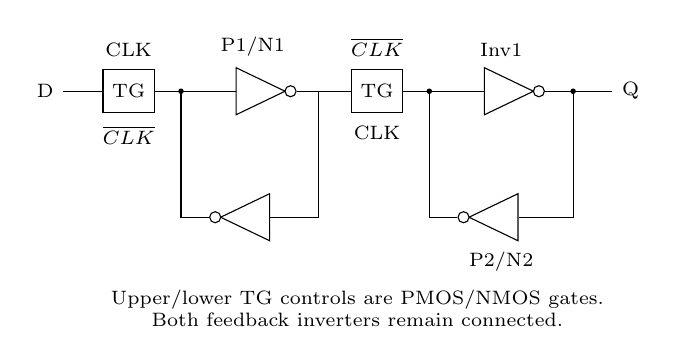
\begin{tikzpicture}[x=.83cm,y=.8cm,font=\scriptsize]
\node[draw,minimum width=.6cm,minimum height=.55cm](t1)at(.7,2.5){TG};\draw(-.3,2.5)node[left]{D}--(t1.west);\node[above]at(.7,2.9){CLK};\node[below]at(.7,2.1){$\overline{CLK}$};
\node[not gate US,draw,minimum width=.7cm](i1)at(2.6,2.5){};\draw(t1.east)--(i1.input);\node[above]at(2.6,2.9){P1/N1};\node[not gate US,draw,rotate=180,minimum width=.7cm](f1)at(2.6,.5){};\draw(i1.output)--(3.6,2.5)--(3.6,.5)--(f1.input);\draw(f1.output)--(1.5,.5)--(1.5,2.5);\fill(1.5,2.5)circle(1pt);
\node[draw,minimum width=.6cm,minimum height=.55cm](t2)at(4.5,2.5){TG};\draw(3.6,2.5)--(t2.west);\node[above]at(4.5,2.9){$\overline{CLK}$};\node[below]at(4.5,2.1){CLK};
\node[not gate US,draw,minimum width=.7cm](i2)at(6.4,2.5){};\draw(t2.east)--(i2.input);\node[above]at(6.4,2.9){Inv1};\draw(i2.output)--(8.1,2.5)node[right]{Q};\node[not gate US,draw,rotate=180,minimum width=.7cm](f2)at(6.4,.5){};\node[below]at(6.4,.1){P2/N2};\draw(7.5,2.5)--(7.5,.5)--(f2.input);\draw(f2.output)--(5.3,.5)--(5.3,2.5);\fill(5.3,2.5)circle(1pt);\fill(7.5,2.5)circle(1pt);\node[align=center]at(4.2,-.95){Upper/lower TG controls are PMOS/NMOS gates.\\Both feedback inverters remain connected.};\end{tikzpicture}\end{center}
\textbf{(a)} The first TG has PMOS gate CLK and NMOS gate $\overline{CLK}$, so the master is transparent while CLK=0. The second TG is transparent while CLK=1. At the rising edge, the master closes and the slave opens. There are two data inversions, so it is a \textbf{rising-edge D register}, $Q=D$ for the value held at that edge, provided writing can overcome the permanently connected feedback inverters.

\textbf{(b)} When the slave is being written high, P1 pulls up through $R_{TG}$ against feedback N2:
\[V_{slave,H}=V_{DD}\frac{R_{N2}}{R_{P1}+R_{TG}+R_{N2}}>\frac{V_{DD}}2
\quad\Longrightarrow\quad\boxed{R_{N2}>R_{P1}+R_{TG}}.\]
When it is being written low, N1 pulls down through $R_{TG}$ against feedback P2:
\[V_{slave,L}=V_{DD}\frac{R_{N1}+R_{TG}}{R_{P2}+R_{N1}+R_{TG}}<\frac{V_{DD}}2
\quad\Longrightarrow\quad\boxed{R_{P2}>R_{N1}+R_{TG}}.\]
Thus P2/N2 must be weaker (higher resistance) than the respective writing path. Equality gives zero DC switching margin, so strict inequalities are preferable. The master's analogous ratios must also permit writing; only P2/N2 are requested. The student's corresponding two divider inequalities are essentially correct, apart from using non-strict equal-bound comparisons.
\small Verification: verify.py independently checks complementary pull-downs, shared-N3 width equations, clock capacitance, state-correlated NP resistances, charge conservation, timing paths, skew/hold repairs, pipeline cycle alignment, and resistor inequalities. Q7's missing upper-threshold datum is recorded rather than fabricated.\end{document}
